\chapter{Meiosis dan Pengocokan Genetik}\label{ch:g12:meiosis-genetic-shuffling}

Dua orang tua, yang masing-masing punya 46 \omterm{def:g11:cell-cycle-mitosis:chromosome}{kromosom}, menghasilkan
seorang anak dengan 46 --- bukan 92. Di suatu tempat antara tubuh orang
tuanya dan anaknya, cacahnya dibagi dua, dan dibagi dua dengan cara
yang membagikan kepada tiap anaknya satu kartu yang tidak pernah
dipegang saudaranya: orang tua yang sama, empat puluh tahun beranak,
dan tidak ada dua yang serupa kecuali kembar identik. Pembagian duanya
adalah pembelahan khusus yang disebut \omterm{def:g12:meiosis-genetic-shuffling:meiosis}{meiosis}; pembagian kartunya
adalah apa yang diperbuatnya pada \omterm{def:g11:cell-cycle-mitosis:chromosome}{kromosomnya} di sepanjang jalan. Bab
ini mengikuti satu \omterm{def:g10:cells-common-unit:cell}{sel} sepanjang \omterm{def:g12:meiosis-genetic-shuffling:meiosis}{meiosis}, menghitung gabungan yang
dapat dihasilkannya, dan membaca hasil persilangan yang menyingkapkan,
dari luar, apa yang terjadi di dalam.

\section{Membagi dua perangkatnya}

\begin{definition}[Diploid, haploid, dan meiosis]\label{def:g12:meiosis-genetic-shuffling:meiosis}
\omterm{def:g10:cells-common-unit:cell}{Sel} yang membawa dua salinan tiap \omterm{def:g11:cell-cycle-mitosis:chromosome}{kromosomnya} --- satu dari tiap orang
tuanya, keduanya membentuk sepasang \emph{kromosom homolog} --- bersifat
\emph{diploid}\index{diploid}, yang ditulis $2n$ ($2n = 46$ pada
manusia). \omterm{def:g10:cells-common-unit:cell}{Sel} yang membawa satu salinan tiap \omterm{def:g11:cell-cycle-mitosis:chromosome}{kromosomnya} bersifat
\emph{haploid}\index{haploid}, yang ditulis $n$.
\emph{Meiosis}\index{meiosis} adalah runtunan dua pembelahan yang
dengannya satu \omterm{def:g10:cells-common-unit:cell}{sel} diploid, setelah satu \omterm{def:g11:dna-replication:replication}{replikasi DNA-nya},
menghasilkan empat \omterm{def:g10:cells-common-unit:cell}{sel} haploid --- yaitu gamet, atau bakalnya.
\emph{Pembuahan} menyatukan dua gamet haploid dan memulihkan bilangan
diploidnya: pergantian meiosis dan pembuahan adalah daur setiap \omterm{def:g10:biodiversity-scales:species}{spesies}
yang berkembang biak secara seksual.
\end{definition}

\begin{proposition}[Kedua pembelahannya]\label{prop:g12:meiosis-genetic-shuffling:divisions}
Sebelum \omterm{def:g12:meiosis-genetic-shuffling:meiosis}{meiosis}, \omterm{def:g10:universal-dna:information}{DNA-nya} direplikasi: tiap \omterm{def:g11:cell-cycle-mitosis:chromosome}{kromosomnya} punya dua
\omterm{def:g11:cell-cycle-mitosis:chromosome}{kromatid}. Lalu:
\begin{itemize}
  \item \emph{Pembelahan pertama} (\omterm{def:g12:meiosis-genetic-shuffling:meiosis}{meiosis} I, \emph{reduksi}): \omterm{def:g11:cell-cycle-mitosis:chromosome}{kromosom}
        homolognya berpasangan, dua demi dua, pada khatulistiwanya;
        anggota tiap pasangannya ditarik ke kutub yang berlawanan. Tiap
        \omterm{def:g10:cells-common-unit:cell}{sel} anaknya menerima \emph{satu \omterm{def:g11:cell-cycle-mitosis:chromosome}{kromosom} dari tiap pasangan},
        yang masih terbuat dari dua \omterm{def:g11:cell-cycle-mitosis:chromosome}{kromatid}: $n$ \omterm{def:g11:cell-cycle-mitosis:chromosome}{kromosom}, dengan \omterm{def:g10:universal-dna:information}{DNA}
        sebanyak $q$ (yaitu jumlah pada \omterm{def:g10:cells-common-unit:cell}{sel} \omterm{def:g12:meiosis-genetic-shuffling:meiosis}{diploid} sebelum replikasinya).
  \item \emph{Pembelahan kedua} (\omterm{def:g12:meiosis-genetic-shuffling:meiosis}{meiosis} II, \emph{ekuasi}): seperti
        sebuah \omterm{def:g11:cell-cycle-mitosis:cycle}{mitosis}, \omterm{def:g11:cell-cycle-mitosis:chromosome}{kromatid} tiap \omterm{def:g11:cell-cycle-mitosis:chromosome}{kromosomnya} memisah. Tiap \omterm{def:g10:cells-common-unit:cell}{sel} dari
        keempatnya menerima $n$ \omterm{def:g11:cell-cycle-mitosis:chromosome}{kromosom} berkromatid tunggal, dengan \omterm{def:g10:universal-dna:information}{DNA}
        sebanyak $q/2$.
\end{itemize}
Pembelahan pertamanya membagi dua jumlah \omterm{def:g11:cell-cycle-mitosis:chromosome}{kromosomnya}; pembelahan
keduanya membagi dua jumlah \omterm{def:g10:universal-dna:information}{DNA-nya} kembali menjadi satu \omterm{def:g11:cell-cycle-mitosis:chromosome}{kromatid} tiap
\omterm{def:g11:cell-cycle-mitosis:chromosome}{kromosom}.
\end{proposition}
\admitted

\begin{omfigure}
\begin{tikzpicture}[font=\small, line cap=round]
  \tikzset{cellb/.style={draw, thick, fill=omDef!5, rounded corners=9pt, minimum width=2.5cm, minimum height=2.5cm},
           ma/.style={line width=3pt, omDef!80}, mb/.style={line width=3pt, omThm!80},
           mA/.style={line width=3pt, omDef!35}, mB/.style={line width=3pt, omThm!35}, cen/.style={fill=black}}
  % panel 1: diploid cell after S: two pairs (long pair blue, short pair red); paternal dark, maternal pale
  \begin{scope}
    \node[cellb] at (0,0) {};
    \draw[ma] (-0.75,0.7) .. controls (-0.62,0.1) .. (-0.75,-0.5); \draw[ma] (-0.49,0.7) .. controls (-0.62,0.1) .. (-0.49,-0.5); \fill[cen] (-0.62,0.1) circle (1.6pt);
    \draw[mA] (-0.2,0.7) .. controls (-0.07,0.1) .. (-0.2,-0.5); \draw[mA] (0.06,0.7) .. controls (-0.07,0.1) .. (0.06,-0.5); \fill[cen] (-0.07,0.1) circle (1.6pt);
    \draw[mb] (0.4,0.45) .. controls (0.53,0.1) .. (0.4,-0.25); \draw[mb] (0.66,0.45) .. controls (0.53,0.1) .. (0.66,-0.25); \fill[cen] (0.53,0.1) circle (1.6pt);
    \draw[mB] (0.9,0.45) .. controls (1.03,0.1) .. (0.9,-0.25); \draw[mB] (1.16,0.45) .. controls (1.03,0.1) .. (1.16,-0.25); \fill[cen] (1.03,0.1) circle (1.6pt);
    \node[anchor=north, align=center, font=\scriptsize, text width=3.05cm] at (0,-1.35) {setelah replikasi:\\ $2n = 4$, DNA $2q$};
  \end{scope}
  % panel 2: metaphase I: pairs on the equator
  \begin{scope}[xshift=3.2cm]
    \node[cellb] at (0,0) {};
    \draw[dashed, gray] (-1.1,0) -- (1.1,0);
    \draw[ma] (-0.7,0.55) .. controls (-0.57,0.1) .. (-0.7,-0.35); \draw[ma] (-0.44,0.55) .. controls (-0.57,0.1) .. (-0.44,-0.35); \fill[cen] (-0.57,0.15) circle (1.6pt);
    \draw[mA] (-0.7,-0.05) .. controls (-0.57,-0.5) .. (-0.7,-0.95); \draw[mA] (-0.44,-0.05) .. controls (-0.57,-0.5) .. (-0.44,-0.95); \fill[cen] (-0.57,-0.15) circle (1.6pt);
    \draw[mb] (0.45,0.5) .. controls (0.58,0.2) .. (0.45,-0.1); \draw[mb] (0.71,0.5) .. controls (0.58,0.2) .. (0.71,-0.1); \fill[cen] (0.58,0.15) circle (1.6pt);
    \draw[mB] (0.45,0.1) .. controls (0.58,-0.2) .. (0.45,-0.5); \draw[mB] (0.71,0.1) .. controls (0.58,-0.2) .. (0.71,-0.5); \fill[cen] (0.58,-0.15) circle (1.6pt);
    \node[anchor=north, align=center, font=\scriptsize, text width=3.05cm] at (0,-1.35) {meiosis I: pasangan\\ homolog pada khatulistiwanya};
  \end{scope}
  % panel 3: two cells after MI, each n=2 with two chromatids
  \begin{scope}[xshift=6.4cm]
    \node[cellb, minimum height=1.15cm] at (0,0.7) {};
    \node[cellb, minimum height=1.15cm] at (0,-0.7) {};
    \draw[ma] (-0.55,1.15) .. controls (-0.42,0.7) .. (-0.55,0.25); \draw[ma] (-0.29,1.15) .. controls (-0.42,0.7) .. (-0.29,0.25); \fill[cen] (-0.42,0.7) circle (1.6pt);
    \draw[mB] (0.35,1.0) .. controls (0.48,0.7) .. (0.35,0.4); \draw[mB] (0.61,1.0) .. controls (0.48,0.7) .. (0.61,0.4); \fill[cen] (0.48,0.7) circle (1.6pt);
    \draw[mA] (-0.55,-0.25) .. controls (-0.42,-0.7) .. (-0.55,-1.15); \draw[mA] (-0.29,-0.25) .. controls (-0.42,-0.7) .. (-0.29,-1.15); \fill[cen] (-0.42,-0.7) circle (1.6pt);
    \draw[mb] (0.35,-0.4) .. controls (0.48,-0.7) .. (0.35,-1.0); \draw[mb] (0.61,-0.4) .. controls (0.48,-0.7) .. (0.61,-1.0); \fill[cen] (0.48,-0.7) circle (1.6pt);
    \node[anchor=north, align=center, font=\scriptsize, text width=3.05cm] at (0,-1.35) {dua sel: $n = 2$,\\ dua kromatid, DNA $q$};
  \end{scope}
  % panel 4: four cells after MII, single chromatids
  \begin{scope}[xshift=9.6cm]
    \foreach \y in {1.05,0.35,-0.35,-1.05} \node[cellb, minimum height=0.6cm, minimum width=2.3cm] at (0,\y) {};
    \draw[ma] (-0.5,1.3) -- (-0.5,0.8); \fill[cen] (-0.5,1.05) circle (1.4pt); \draw[mB] (0.4,1.22) -- (0.4,0.88); \fill[cen] (0.4,1.05) circle (1.4pt);
    \draw[ma] (-0.5,0.6) -- (-0.5,0.1); \fill[cen] (-0.5,0.35) circle (1.4pt); \draw[mB] (0.4,0.52) -- (0.4,0.18); \fill[cen] (0.4,0.35) circle (1.4pt);
    \draw[mA] (-0.5,-0.1) -- (-0.5,-0.6); \fill[cen] (-0.5,-0.35) circle (1.4pt); \draw[mb] (0.4,-0.18) -- (0.4,-0.52); \fill[cen] (0.4,-0.35) circle (1.4pt);
    \draw[mA] (-0.5,-0.8) -- (-0.5,-1.3); \fill[cen] (-0.5,-1.05) circle (1.4pt); \draw[mb] (0.4,-0.88) -- (0.4,-1.22); \fill[cen] (0.4,-1.05) circle (1.4pt);
    \node[anchor=north, align=center, font=\scriptsize, text width=3.05cm] at (0,-1.45) {empat gamet: $n = 2$,\\ satu kromatid, DNA $q/2$};
  \end{scope}
\end{tikzpicture}

{\small \omterm{def:g12:meiosis-genetic-shuffling:meiosis}{Meiosis} dalam \omterm{def:g10:cells-common-unit:cell}{sel} dengan dua pasang \omterm{def:g11:cell-cycle-mitosis:chromosome}{kromosom} ($2n = 4$); warna
gelap dan pucatnya menandai kedua anggota tiap pasangannya, dari kedua
orang tuanya. Pembelahan pertamanya memisahkan homolognya, yang kedua
memisahkan \omterm{def:g11:cell-cycle-mitosis:chromosome}{kromatidnya}. Di sini \omterm{def:g11:cell-cycle-mitosis:chromosome}{kromosom} panjang yang gelap pergi
bersama \omterm{def:g11:cell-cycle-mitosis:chromosome}{kromosom} pendek yang pucat: salah satu dari dua pembagian yang mungkin.}
\end{omfigure}

\begin{omfigure}
\begin{tikzpicture}
\begin{axis}[
  width=0.88\linewidth, height=5.2cm,
  axis x line=bottom, axis y line=left,
  xmin=0, xmax=10, ymin=0, ymax=2.7,
  xlabel={waktu}, ylabel={DNA tiap sel},
  xlabel style={font=\small, at={(axis description cs:0.5,-0.1)}, anchor=north},
  ylabel style={font=\small},
  tick label style={font=\small}, xtick=\empty,
  ytick={0.5,1,2}, yticklabels={$q/2$, $q$, $2q$},
  clip=false,
]
\addplot[thick, omDef] coordinates {(0,1) (2,1) (4,2) (5.9,2) (6,1) (7.9,1) (8,0.5) (10,0.5)};
\draw[dashed, gray] (axis cs:2,0) -- (axis cs:2,2.2); \draw[dashed, gray] (axis cs:4,0) -- (axis cs:4,2.2);
\draw[dashed, gray] (axis cs:6,0) -- (axis cs:6,2.2); \draw[dashed, gray] (axis cs:8,0) -- (axis cs:8,2.2);
\node[font=\small, anchor=south] at (axis cs:1,2.25) {$2n$, $q$};
\node[font=\small, anchor=south] at (axis cs:3,2.25) {fase S};
\node[font=\small, anchor=south] at (axis cs:5,2.25) {$2n$, $2q$};
\node[font=\small, anchor=south, omThm] at (axis cs:6,2.45) {meiosis tahap I};
\node[font=\small, anchor=south] at (axis cs:7,2.25) {$n$, $q$};
\node[font=\small, anchor=south, omThm] at (axis cs:8,2.45) {meiosis tahap II};
\node[font=\small, anchor=south] at (axis cs:9,2.25) {$n$, $q/2$};
\end{axis}
\end{tikzpicture}

{\small \omterm{def:g10:universal-dna:information}{DNA} tiap \omterm{def:g10:cells-common-unit:cell}{sel} sepanjang \omterm{def:g12:meiosis-genetic-shuffling:meiosis}{meiosis}. Satu replikasi, lalu dua
pembelahan tanpa replikasi di antaranya: gametnya memuat seperempat \omterm{def:g10:universal-dna:information}{DNA}
yang dimuat \omterm{def:g10:cells-common-unit:cell}{sel} induknya setelah S, dan separuh dari yang dimuat \omterm{def:g10:cells-common-unit:cell}{sel}
\omterm{def:g12:meiosis-genetic-shuffling:meiosis}{diploid} dalam keadaan istirahat.}
\end{omfigure}

\begin{example}[Angka manusia]\label{ex:g12:meiosis-genetic-shuffling:numbers}
\omterm{def:g10:cells-common-unit:cell}{Sel} kelamin sebuah testis, $2n = 46$, mereplikasi diri menjadi 46
\omterm{def:g11:cell-cycle-mitosis:chromosome}{kromosom} berkromatid dua ($2q$); setelah \omterm{def:g12:meiosis-genetic-shuffling:meiosis}{meiosis} I, dua \omterm{def:g10:cells-common-unit:cell}{sel} berisi 23
\omterm{def:g11:cell-cycle-mitosis:chromosome}{kromosom} berkromatid dua ($q$); setelah \omterm{def:g12:meiosis-genetic-shuffling:meiosis}{meiosis} II, empat \omterm{def:g10:cells-common-unit:cell}{sel} sperma
berisi 23 \omterm{def:g11:cell-cycle-mitosis:chromosome}{kromosom} berkromatid tunggal ($q/2$). Pada pembuahannya, $23 + 23 =
46$ dan $q/2 + q/2 = q$: zigotnya kembali menjadi \omterm{def:g10:cells-common-unit:cell}{sel}
\omterm{def:g12:meiosis-genetic-shuffling:meiosis}{diploid} dalam keadaan istirahat. Dalam ovariumnya, pembelahan yang sama
menghasilkan satu \omterm{def:g10:cells-common-unit:cell}{sel} telur besar dan tiga \omterm{def:g10:cells-common-unit:cell}{sel} mungil yang dibuang;
hitungannya serupa.
\end{example}

\section{Pengocokannya}

\begin{proposition}[Pemilahan bebas]\label{prop:g12:meiosis-genetic-shuffling:assortment}
Pada metafase I, tiap pasangan homolognya berbaris pada khatulistiwanya
tanpa bergantung pada pasangan lainnya: anggota mana dari sebuah
pasangan yang pergi ke kutub yang mana diputuskan kebetulan, pasangan
demi pasangan. Karena itu \omterm{def:g10:cells-common-unit:cell}{sel} dengan $n$ pasangan dapat menghasilkan
$2^n$ gabungan \omterm{def:g11:cell-cycle-mitosis:chromosome}{kromosom} ayah dan ibu yang berbeda dalam gametnya ---
$2^{23} \approx \num{8.4e6}$ pada manusia. Pembuahan, yang menyatukan
dua gamet semacam itu secara acak, memberi $2^{23}
\times 2^{23} \approx \num{7e13}$ gabungan \omterm{def:g11:cell-cycle-mitosis:chromosome}{kromosom} bagi anak sepasang suami istri,
sebelum sumber keragaman lainnya dihitung.
\end{proposition}
\admitted

\begin{proposition}[Pindah silang]\label{prop:g12:meiosis-genetic-shuffling:crossingover}
Ketika homolognya berpasangan, pada awal \omterm{def:g12:meiosis-genetic-shuffling:meiosis}{meiosis} I, dua \omterm{def:g11:cell-cycle-mitosis:chromosome}{kromatid} yang
bukan saudara putus pada titik yang sama lalu bersambung menyilang:
itulah \emph{pindah silang}\index{pindah silang}. Tiap \omterm{def:g11:cell-cycle-mitosis:chromosome}{kromatidnya} di
seberang titik pertukarannya kini membawa \omterm{def:g10:universal-dna:gene}{alel} homolog yang lain.
Karena itu \omterm{def:g11:cell-cycle-mitosis:chromosome}{kromosom} yang mencapai gametnya bukanlah \omterm{def:g11:cell-cycle-mitosis:chromosome}{kromosom} orang
tuanya melainkan \omterm{def:g11:cell-cycle-mitosis:chromosome}{kromosom} yang \emph{tergabung ulang}, yang mencampur
di sepanjang panjangnya \omterm{def:g10:universal-dna:gene}{alel} yang diterima dari kedua kakek neneknya.
Satu sampai tiga pertukaran terjadi pada tiap pasangan pada tiap
\omterm{def:g12:meiosis-genetic-shuffling:meiosis}{meiosis}, pada kedudukan yang berubah-ubah: dalam praktiknya, jumlah
gamet yang mungkin tidak terbatas.
\end{proposition}
\begin{proof}[Bukti percobaan]
Di bawah mikroskop, homolog yang berpasangan dalam \omterm{def:g12:meiosis-genetic-shuffling:meiosis}{meiosis} I
memperlihatkan titik yang menyilang, yaitu \emph{kiasma}, tempat dua
\omterm{def:g11:cell-cycle-mitosis:chromosome}{kromatid} tampak bertukar pasangan. Persilangan yang kedua \omterm{def:g10:universal-dna:gene}{gennya}
terletak pada \omterm{def:g11:cell-cycle-mitosis:chromosome}{kromosom} yang sama memberi, di antara keturunannya,
sebagian kecil yang membawa gabungan baru \omterm{def:g10:universal-dna:gene}{alel} kedua \omterm{def:g10:universal-dna:gene}{gennya} ---
gabungan yang tidak dibawa satu pun orang tuanya --- dalam perbandingan
yang bergantung pada jarak antara \omterm{def:g10:universal-dna:gene}{gennya}; \omterm{def:g10:universal-dna:gene}{gen} yang berjauhan pada
sebuah \omterm{def:g11:cell-cycle-mitosis:chromosome}{kromosom} bergabung ulang sesering \omterm{def:g10:universal-dna:gene}{gen} pada \omterm{def:g11:cell-cycle-mitosis:chromosome}{kromosom} yang
berbeda. Penanda molekuler yang diikuti dalam beberapa keluarga
memperlihatkan ruas tiap \omterm{def:g11:cell-cycle-mitosis:chromosome}{kromosomnya} berganti asal kakek neneknya pada
satu atau dua titik tiap \omterm{def:g11:cell-cycle-mitosis:chromosome}{kromosom} tiap keturunan.
\end{proof}

\begin{omfigure}
\begin{tikzpicture}[font=\small, line cap=round, >=Stealth]
  \tikzset{p/.style={line width=4pt, omDef!80}, m/.style={line width=4pt, omThm!70}}
  % before: two homologues, each two chromatids; alleles A/a, B/b
  \draw[p] (0,0) -- (0,3); \draw[p] (0.35,0) -- (0.35,3);
  \draw[m] (0.9,0) -- (0.9,3); \draw[m] (1.25,0) -- (1.25,3);
  \foreach \x in {0,0.35} { \node[font=\scriptsize, anchor=east, xshift=-1pt] at (\x,2.6) {}; }
  \node[font=\scriptsize, omDef!80!black, anchor=east] at (-0.15,2.6) {$A$};
  \node[font=\scriptsize, omDef!80!black, anchor=east] at (-0.15,0.5) {$B$};
  \node[font=\scriptsize, omThm!80!black, anchor=west] at (1.4,2.6) {$a$};
  \node[font=\scriptsize, omThm!80!black, anchor=west] at (1.4,0.5) {$b$};
  \node[anchor=north, align=center] at (0.62,-0.2) {homolog yang berpasangan\\ (masing-masing dua kromatid)};
  \draw[->, thick] (2.4,1.5) -- (3.4,1.5);
  % during: chiasma between the two inner chromatids at y=1.5
  \begin{scope}[xshift=4.2cm]
    \draw[p] (0,0) -- (0,3);
    \draw[p] (0.35,3) -- (0.35,1.6) -- (0.9,1.4) -- (0.9,0);
    \draw[m] (0.9,3) -- (0.9,1.6) -- (0.35,1.4) -- (0.35,0);
    \draw[m] (1.25,0) -- (1.25,3);
    \node[anchor=north, align=center] at (0.62,-0.2) {kiasma: dua kromatid\\ putus lalu bersambung menyilang};
  \end{scope}
  \draw[->, thick] (6.6,1.5) -- (7.6,1.5);
  % after: four chromatids separated
  \begin{scope}[xshift=8.4cm]
    \draw[p] (0,0) -- (0,3);
    \draw[p] (0.5,3) -- (0.5,1.5); \draw[m] (0.5,1.5) -- (0.5,0);
    \draw[m] (1.0,3) -- (1.0,1.5); \draw[p] (1.0,1.5) -- (1.0,0);
    \draw[m] (1.5,0) -- (1.5,3);
    \node[font=\scriptsize, anchor=south] at (0,3.05) {$AB$};
    \node[font=\scriptsize, anchor=south] at (0.5,3.05) {$Ab$};
    \node[font=\scriptsize, anchor=south] at (1.0,3.05) {$aB$};
    \node[font=\scriptsize, anchor=south] at (1.5,3.05) {$ab$};
    \node[anchor=north, align=center] at (0.75,-0.2) {empat gamet: dua tetua,\\ dua tergabung ulang};
  \end{scope}
\end{tikzpicture}

{\small \omterm{prop:g12:meiosis-genetic-shuffling:crossingover}{Pindah silang} antara dua \omterm{def:g10:universal-dna:gene}{gen} $A$ dan $B$ pada \omterm{def:g11:cell-cycle-mitosis:chromosome}{kromosom} yang
sama. Dua dari keempat \omterm{def:g11:cell-cycle-mitosis:chromosome}{kromatidnya} menukar ujungnya; dari keempat
gametnya, dua membawa gabungan tetuanya ($AB$, $ab$) dan dua membawa
gabungan yang baru ($Ab$, $aB$).}
\end{omfigure}

\begin{omfigure}
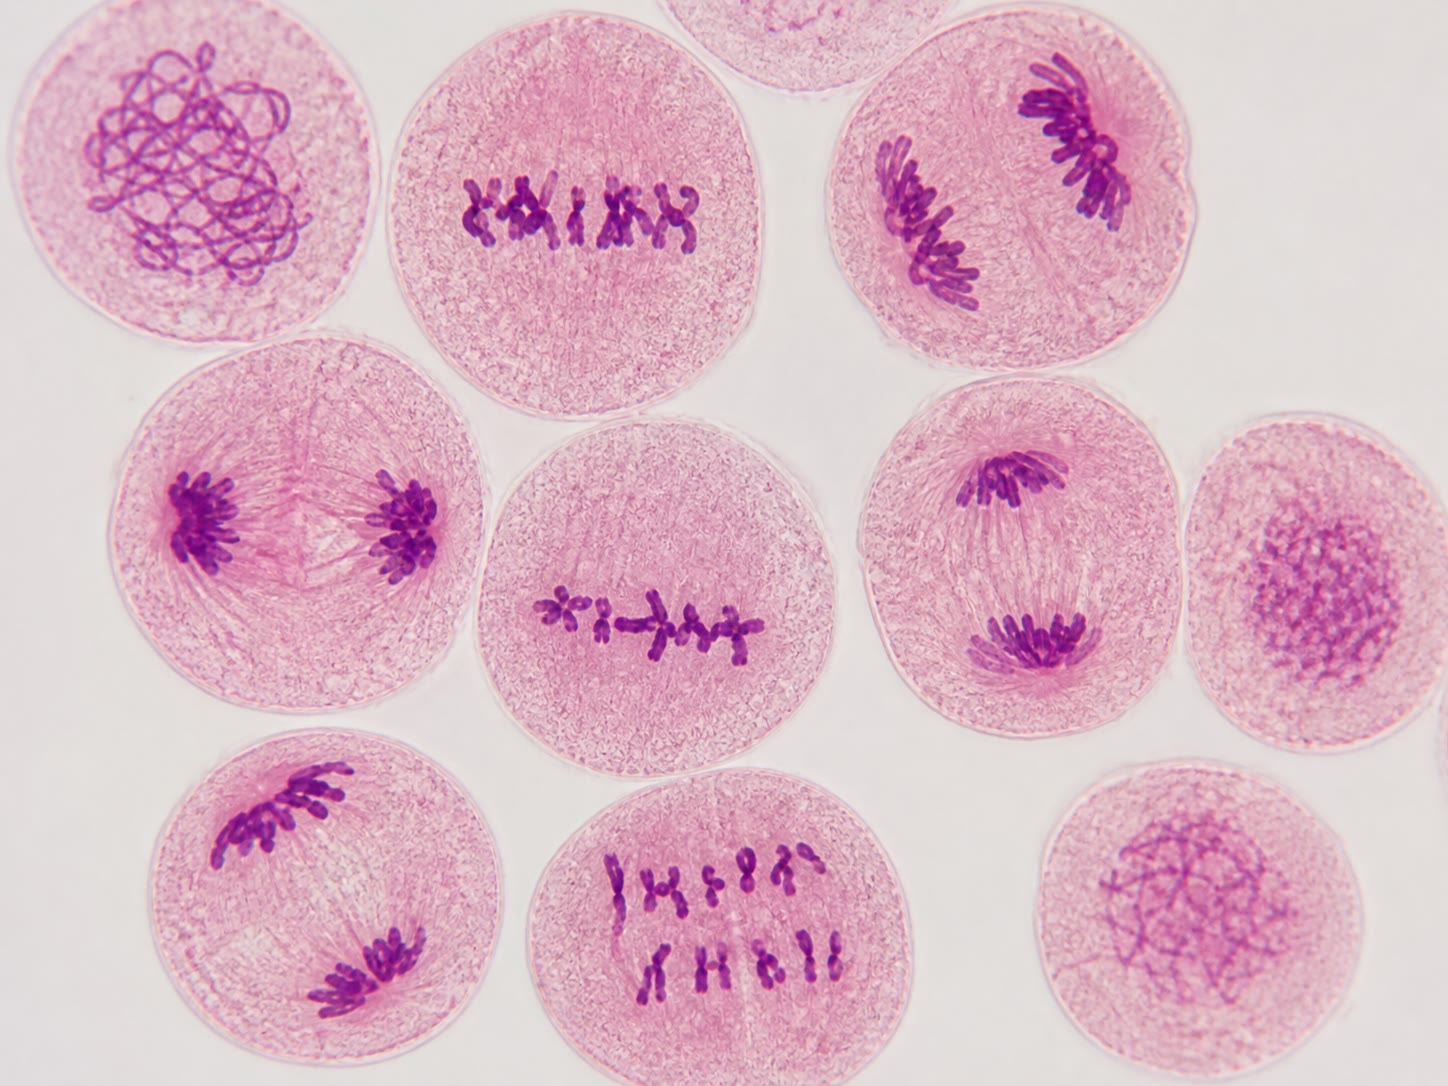
\includegraphics[width=0.56\linewidth]{images/book2/ai/g12-meiosis-lily-anther.jpg}

{\small \omterm{def:g10:cells-common-unit:cell}{Sel} kepala sari bunga bakung dalam \omterm{def:g12:meiosis-genetic-shuffling:meiosis}{meiosis}, yang diwarnai: pada
sebagian, homolog yang berpasangan berbaris melintasi tengah \omterm{def:g10:cells-common-unit:cell}{selnya};
pada sebagian lagi, homolognya telah ditarik ke kedua kutubnya. Tahap
skemanya, yang terlihat pada jaringan pembuat serbuk sari.}
\end{omfigure}

\begin{example}[Tiga sumber keragaman, secara berurutan]\label{ex:g12:meiosis-genetic-shuffling:sources}
Seorang anak dari dua orang tua baru dalam tiga hal: \omterm{prop:g12:meiosis-genetic-shuffling:crossingover}{pindah silang}
membangun ulang tiap \omterm{def:g11:cell-cycle-mitosis:chromosome}{kromosom} tiap gametnya dari kedua salinan kakek
neneknya; pemilahan bebas membagikan satu \omterm{def:g11:cell-cycle-mitosis:chromosome}{kromosom} yang tergabung ulang
dari tiap pasangannya ke dalam gametnya, di antara $2^{23}$ pembagian;
pembuahan menggabungkan satu gamet semacam itu dengan gamet lain yang
diundi dari $2^{23}$ milik orang tuanya yang lain. \omterm{def:g11:mutations:mutation}{Mutasi}, yang
menciptakan \omterm{def:g10:universal-dna:gene}{alel} yang sedang dikocok itu, bekerja pada skala waktu yang
jauh lebih lambat: pengocokannyalah yang membuat tiap keturunan baru
dari tumpukan kartu yang sama.
\end{example}

\section{Membaca pengocokannya dalam sebuah persilangan}

\begin{omfigure}
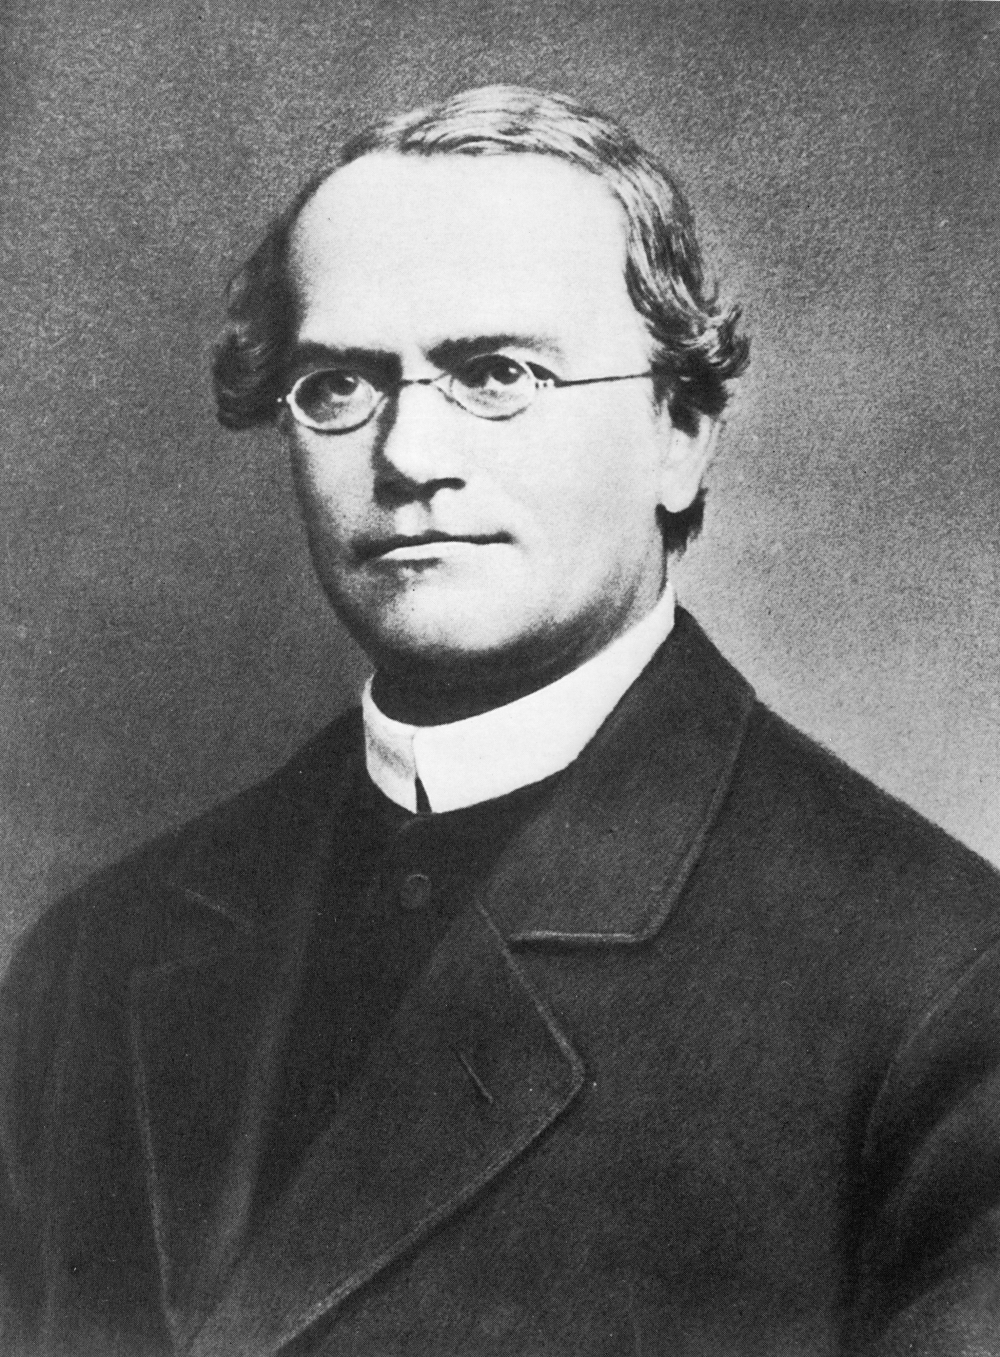
\includegraphics[width=0.3\linewidth]{images/book2/mendel.jpg}

{\small Gregor Mendel, yang menghitung keturunan persilangan kacang ercis di kebun biara pada 1860-an dan menemukan nisbahnya --- 3:1 bagi satu ciri, 9:3:3:1 bagi dua ciri --- yang dihasilkan \omterm{def:g12:meiosis-genetic-shuffling:meiosis}{meiosis}, yang tak dikenalnya. Foto, domain publik.}
\end{omfigure}

\begin{method}[Uji silang]\label{met:g12:meiosis-genetic-shuffling:testcross}
Untuk melihat gamet apa yang dibuat seorang individu, silangkan ia
dengan pasangan yang hanya membawa \omterm{def:g10:universal-dna:gene}{alel} \omterm{def:g11:genes-and-disease:genetic}{resesif} (sebuah \emph{uji
silang}): tiap keturunannya lalu memperlihatkan persis \omterm{def:g10:universal-dna:gene}{alel} yang dibawa
gamet tetua yang diuji. Untuk dua \omterm{def:g10:universal-dna:gene}{gen}, dengan tetua yang diuji $AaBb$
dan pasangannya $aabb$:
\begin{enumerate}
  \item Hitung keempat macam keturunannya: $AB$, $Ab$, $aB$, $ab$
        (masing-masing juga membawa $ab$ dari pasangannya).
  \item Jika keempatnya sama seringnya ($1:1:1:1$), \omterm{def:g10:universal-dna:gene}{gennya} terletak
        pada \omterm{def:g11:cell-cycle-mitosis:chromosome}{kromosom} yang berbeda dan terpilah bebas.
  \item Jika dua macamnya (gabungan tetuanya) jauh lebih lazim daripada
        dua macam lainnya (rekombinannya), \omterm{def:g10:universal-dna:gene}{gennya} terletak pada
        \omterm{def:g11:cell-cycle-mitosis:chromosome}{kromosom} yang sama; rekombinannya berasal dari \omterm{prop:g12:meiosis-genetic-shuffling:crossingover}{pindah silang},
        dan bagiannya mengukur jarak antara \omterm{def:g10:universal-dna:gene}{gennya}.
  \item Rekombinannya selalu menjadi yang sedikit dan selalu hadir
        dalam dua kelas yang sama besar; begitu pula tetuanya.
\end{enumerate}
\end{method}

\begin{example}[Dua persilangan pada lalat buah]\label{ex:g12:meiosis-genetic-shuffling:fly}
Lalat A, yang heterozigot bagi warna tubuh dan bentuk sayapnya, diuji
silang: 254 kelabu-normal, 248 hitam-vestigial, 251 kelabu-vestigial,
247 hitam-normal --- empat kelas yang sama besar, sehingga \omterm{def:g10:universal-dna:gene}{gennya}
berada pada \omterm{def:g11:cell-cycle-mitosis:chromosome}{kromosom} yang berbeda. Lalat B, yang heterozigot bagi warna
tubuh dan warna \omterm{def:g11:the-eye:parts}{matanya}: 412 kelabu-merah, 405 hitam-ungu, 44
kelabu-ungu, 39 hitam-merah --- dua kelas tetua yang masing-masing
sekitar 45\% dan dua kelas rekombinan yang masing-masing sekitar 5\%:
\omterm{def:g10:universal-dna:gene}{gennya} berada pada \omterm{def:g11:cell-cycle-mitosis:chromosome}{kromosom} yang sama, berdekatan, yang terpisahkan
sebuah \omterm{prop:g12:meiosis-genetic-shuffling:crossingover}{pindah silang} pada 9\% \omterm{def:g12:meiosis-genetic-shuffling:meiosis}{meiosisnya}.
\end{example}

\begin{omfigure}
\begin{tikzpicture}[font=\small]
  \draw[thick] (0,0) grid[step=1.4] (5.6,1.4);
  \node[fill=omDef!15, minimum width=1.3cm, minimum height=1.3cm, align=center] at (0.7,0.7) {$AB$\\ 254};
  \node[fill=omDef!15, minimum width=1.3cm, minimum height=1.3cm, align=center] at (2.1,0.7) {$Ab$\\ 251};
  \node[fill=omDef!15, minimum width=1.3cm, minimum height=1.3cm, align=center] at (3.5,0.7) {$aB$\\ 247};
  \node[fill=omDef!15, minimum width=1.3cm, minimum height=1.3cm, align=center] at (4.9,0.7) {$ab$\\ 248};
  \node[anchor=south] at (2.8,1.5) {lalat A: gen yang bebas, $1:1:1:1$};
  \begin{scope}[xshift=7.4cm]
    \draw[thick] (0,0) grid[step=1.4] (5.6,1.4);
    \node[fill=omProp!25, minimum width=1.3cm, minimum height=1.3cm, align=center] at (0.7,0.7) {$AB$\\ 412};
    \node[fill=omThm!20, minimum width=1.3cm, minimum height=1.3cm, align=center] at (2.1,0.7) {$Ab$\\ 44};
    \node[fill=omThm!20, minimum width=1.3cm, minimum height=1.3cm, align=center] at (3.5,0.7) {$aB$\\ 39};
    \node[fill=omProp!25, minimum width=1.3cm, minimum height=1.3cm, align=center] at (4.9,0.7) {$ab$\\ 405};
    \node[anchor=south] at (2.8,1.5) {lalat B: gen yang terpaut, tetua $\gg$ rekombinan};
  \end{scope}
\end{tikzpicture}

{\small Gamet dua lalat heterozigot, yang terbaca dari uji silangnya.
Kelas yang sama besar berarti pemilahan bebas; dua kelas besar dan dua
kelas kecil berarti \omterm{def:g10:universal-dna:gene}{gennya} terpaut, dengan kelas kecilnya dihasilkan
\omterm{prop:g12:meiosis-genetic-shuffling:crossingover}{pindah silang}.}
\end{omfigure}

\section{Ketika pengocokannya keliru}

\begin{proposition}[Kesalahan meiosis]\label{prop:g12:meiosis-genetic-shuffling:errors}
Sesekali sepasang homolog gagal memisah pada \omterm{def:g12:meiosis-genetic-shuffling:meiosis}{meiosis} I, atau dua
\omterm{def:g11:cell-cycle-mitosis:chromosome}{kromatid} pada \omterm{def:g12:meiosis-genetic-shuffling:meiosis}{meiosis} II: satu gamet menerima dua salinan sebuah
\omterm{def:g11:cell-cycle-mitosis:chromosome}{kromosom} dan gamet lain tidak menerima satu pun. Setelah dibuahi,
keduanya memberi zigot dengan tiga salinan (\emph{trisomi}) atau satu
(\emph{monosomi}). Sebagian besar zigot semacam itu tidak berkembang;
yang berkembang membawa seperangkat ciri yang khas. Trisomi 21 (sekitar
satu kelahiran dari 700) menyebabkan ketidakmampuan berpikir dan cacat
jantung serta menjadi yang terlazim; frekuensinya naik tajam seiring
umur ibunya. \omterm{prop:g12:meiosis-genetic-shuffling:crossingover}{Pindah silang} yang tak seimbang --- yaitu \omterm{def:g11:cell-cycle-mitosis:chromosome}{kromatid} yang
menukar ruas yang tak sama --- menghasilkan sebuah \omterm{def:g11:cell-cycle-mitosis:chromosome}{kromosom} dengan \omterm{def:g10:universal-dna:gene}{gen}
yang tergandakan dan sebuah \omterm{def:g11:cell-cycle-mitosis:chromosome}{kromosom} dengan delesi: itulah mekanisme
yang dengannya \omterm{def:g10:universal-dna:gene}{gen} \omterm{def:g11:the-eye:photoreceptors}{opsin} \cref{ch:g11:the-eye} dilipatgandakan, dan
yang dengannya \omterm{def:g10:universal-dna:gene}{gen} baru muncul (\cref{ch:g12:diversification-of-life}).
\end{proposition}
\admitted

\begin{omfigure}
\begin{tikzpicture}
\begin{axis}[
  width=0.84\linewidth, height=5.4cm,
  axis x line=bottom, axis y line=left,
  xmin=18, xmax=47, ymin=0, ymax=40,
  xlabel={umur ibunya (tahun)}, ylabel={trisomi 21 tiap 1000 kelahiran},
  xlabel style={font=\small, at={(axis description cs:0.5,-0.12)}, anchor=north},
  ylabel style={font=\small},
  tick label style={font=\small}, xtick={20,25,30,35,40,45}, ytick={0,10,20,30,40},
]
\addplot[thick, omThm, mark=*, mark size=1.5pt] coordinates
  {(20,0.7) (25,0.8) (30,1.1) (33,1.8) (35,2.9) (37,4.5) (39,7.5) (41,12) (43,20) (45,33)};
\end{axis}
\end{tikzpicture}

{\small Frekuensi trisomi 21 saat lahir terhadap umur ibunya. \omterm{def:g10:cells-common-unit:cell}{Sel}
telurnya terbentuk sebelum perempuannya lahir dan tertahan dalam
\omterm{def:g12:meiosis-genetic-shuffling:meiosis}{meiosis} I selama puluhan tahun; makin lama penungguan itu, makin mungkin
homolognya gagal memisah.}
\end{omfigure}

\begin{example}[Kromosom kelamin yang salah hitung]\label{ex:g12:meiosis-genetic-shuffling:sexchrom}
Sebuah gamet tanpa \omterm{def:g11:becoming-male-female:chromosomes}{kromosom kelamin} yang dibuahi gamet \omterm{def:g11:genes-and-disease:genetic}{pembawa} X
memberi zigot XO: seorang anak perempuan bertubuh pendek yang
ovariumnya tidak berkembang. \omterm{def:g10:cells-common-unit:cell}{Sel} telur XX yang dibuahi sperma Y memberi
XXY: seorang anak lelaki yang testisnya tetap kecil dan tidak membuat
sperma. Pada keduanya, \omterm{prop:g11:becoming-male-female:sry}{SRY} memutuskan gonadnya seperti pada
\cref{ch:g11:becoming-male-female}; jumlah \omterm{def:g11:cell-cycle-mitosis:chromosome}{kromosom} X-nya memutuskan
sebagian besar sisanya, dan itulah sebabnya keduanya menjadi kesalahan
\omterm{def:g11:cell-cycle-mitosis:chromosome}{kromosom} yang paling ringan.
\end{example}

\begin{remark}[Mengapa ada kelamin]\label{rem:g12:meiosis-genetic-shuffling:whysex}
Bakteri menyalin dirinya; sebatang mawar dapat tumbuh dari setek.
Perkembangbiakan seksual lebih mahal --- dua orang tua, \omterm{def:g12:meiosis-genetic-shuffling:meiosis}{meiosis},
pencarian pasangan --- dan hasilnya adalah sekumpulan keturunan yang
masing-masing berbeda dari orang tuanya dan dari satu sama lain. Beda
itulah pokoknya: dalam lingkungan yang berubah, dan melawan parasit
yang berevolusi, populasi berisi individu yang beragam lebih mungkin
memuat sebagian yang selamat daripada populasi berisi salinan.
Pengocokan bab ini adalah bahan mentah yang akan dipilah seleksi pada
dua bab berikutnya.
\end{remark}

\section{Latihan}

\begin{exercise}[$\star$]\label{exo:g12:meiosis-genetic-shuffling:1}
Rumuskan \omterm{def:g12:meiosis-genetic-shuffling:meiosis}{diploid} dan \omterm{def:g12:meiosis-genetic-shuffling:meiosis}{haploid}, dan nyatakan apa yang diperbuat \omterm{def:g12:meiosis-genetic-shuffling:meiosis}{meiosis}
pada jumlah \omterm{def:g11:cell-cycle-mitosis:chromosome}{kromosom} dan pada jumlah \omterm{def:g10:universal-dna:information}{DNA-nya}.
\end{exercise}

\begin{exercise}[$\star$]\label{exo:g12:meiosis-genetic-shuffling:2}
Apa yang memisah pada \omterm{def:g12:meiosis-genetic-shuffling:meiosis}{meiosis} I? Pada \omterm{def:g12:meiosis-genetic-shuffling:meiosis}{meiosis} II? Pembelahan mana yang
menjadi pembelahan reduksinya?
\end{exercise}

\begin{exercise}[$\star$]\label{exo:g12:meiosis-genetic-shuffling:3}
Sebuah \omterm{def:g10:cells-common-unit:cell}{sel} punya $2n = 8$ dan \omterm{def:g10:universal-dna:information}{DNA} $2q$ pada awal \omterm{def:g12:meiosis-genetic-shuffling:meiosis}{meiosisnya}. Sebutkan
jumlah \omterm{def:g11:cell-cycle-mitosis:chromosome}{kromosom} dan jumlah \omterm{def:g10:universal-dna:information}{DNA} \omterm{def:g10:cells-common-unit:cell}{sel} setelah \omterm{def:g12:meiosis-genetic-shuffling:meiosis}{meiosis} I dan setelah
\omterm{def:g12:meiosis-genetic-shuffling:meiosis}{meiosis} II.
\end{exercise}

\begin{exercise}[$\star$]\label{exo:g12:meiosis-genetic-shuffling:4}
Berapa gabungan \omterm{def:g11:cell-cycle-mitosis:chromosome}{kromosom} yang dapat diperlihatkan gamet sebuah \omterm{def:g10:biodiversity-scales:species}{spesies}
dengan $2n = 8$ lewat pemilahan bebas saja?
\end{exercise}

\begin{exercise}[$\star$]\label{exo:g12:meiosis-genetic-shuffling:5}
Apa itu uji silang, dan apa yang disingkapkan bagian keturunan yang
rekombinan?
\end{exercise}

\begin{exercise}[$\star\star$]\label{exo:g12:meiosis-genetic-shuffling:6}
Dari gambar \omterm{def:g10:universal-dna:information}{DNA-nya}, bacalah \omterm{def:g10:universal-dna:information}{DNA} tiap \omterm{def:g10:cells-common-unit:cell}{sel} bagi \omterm{def:g10:cells-common-unit:cell}{sel} dalam \omterm{def:g12:meiosis-genetic-shuffling:meiosis}{meiosis} I,
bagi \omterm{def:g10:cells-common-unit:cell}{sel} di antara kedua pembelahannya, dan bagi sebuah gamet.
Jelaskan mengapa tidak ada fase S di antara pembelahannya.
\end{exercise}

\begin{exercise}[$\star\star$]\label{exo:g12:meiosis-genetic-shuffling:7}
Sebuah uji silang memberi 300 $AB$, 298 $ab$, 302 $Ab$, 300 $aB$.
Apakah \omterm{def:g10:universal-dna:gene}{gennya} terpaut? Apa saja gamet tetuanya?
\end{exercise}

\begin{exercise}[$\star\star$]\label{exo:g12:meiosis-genetic-shuffling:8}
Sebuah uji silang memberi 460 $AB$, 455 $ab$, 42 $Ab$, 43 $aB$. Apakah
\omterm{def:g10:universal-dna:gene}{gennya} terpaut? Kelas mana yang rekombinan, dan berapa bagiannya?
\end{exercise}

\begin{exercise}[$\star\star$]\label{exo:g12:meiosis-genetic-shuffling:9}
Pada gambar \omterm{prop:g12:meiosis-genetic-shuffling:crossingover}{pindah silangnya}, dua gamet mana yang akan kamu peroleh
jika pertukarannya berlangsung \emph{di atas} kedua \omterm{def:g10:universal-dna:gene}{gennya}? Jelaskan.
\end{exercise}

\begin{exercise}[$\star\star$]\label{exo:g12:meiosis-genetic-shuffling:10}
Dari gambar trisominya, bacalah frekuensinya pada umur 25, 35 dan 42
tahun, lalu hitung faktornya antara 25 dan 42.
\end{exercise}

\begin{exercise}[$\star\star$]\label{exo:g12:meiosis-genetic-shuffling:11}
Jelaskan bagaimana gagal berpisah pada \omterm{def:g12:meiosis-genetic-shuffling:meiosis}{meiosis} I berbeda dari gagal
berpisah pada \omterm{def:g12:meiosis-genetic-shuffling:meiosis}{meiosis} II dalam gamet yang dihasilkannya (tinjaulah
keempat \omterm{def:g10:cells-common-unit:cell}{selnya}).
\end{exercise}

\begin{exercise}[$\star\star\star$]\label{exo:g12:meiosis-genetic-shuffling:12}
Dua \omterm{def:g10:universal-dna:gene}{gen} pada \omterm{def:g11:cell-cycle-mitosis:chromosome}{kromosom} yang sama bergabung ulang pada 2\% \omterm{def:g12:meiosis-genetic-shuffling:meiosis}{meiosisnya};
dua \omterm{def:g10:universal-dna:gene}{gen} lain pada \omterm{def:g11:cell-cycle-mitosis:chromosome}{kromosom} yang sama pada 48\%. Jelaskan apa yang
dinyatakan tiap angkanya tentang jaraknya, dan mengapa pasangan yang
kedua berperilaku nyaris seperti \omterm{def:g10:universal-dna:gene}{gen} yang bebas.
\end{exercise}

\begin{exercise}[$\star\star\star$]\label{exo:g12:meiosis-genetic-shuffling:13}
Sebuah tumbuhan punya $2n = 4$, dengan satu pasangnya membawa $A/a$ dan
yang lain $B/b$. Daftarkan seluruh gamet tumbuhan $AaBb$ beserta
frekuensinya, tanpa \omterm{prop:g12:meiosis-genetic-shuffling:crossingover}{pindah silang}; lalu sebutkan apa yang akan diubah
\omterm{prop:g12:meiosis-genetic-shuffling:crossingover}{pindah silangnya}.
\end{exercise}

\begin{exercise}[$\star\star\star$]\label{exo:g12:meiosis-genetic-shuffling:14}
Kembar identik berbagi seluruh \omterm{def:g10:universal-dna:gene}{alelnya}; saudara biasa berbagi
separuhnya rata-rata. Jelaskan ``separuhnya'' itu dengan \omterm{def:g12:meiosis-genetic-shuffling:meiosis}{meiosis} dan
pembuahannya, dan mengapa itu hanya rata-rata.
\end{exercise}

\begin{exercise}[$\star\star\star$]\label{exo:g12:meiosis-genetic-shuffling:15}
Sebagian tumbuhan berkembang biak lewat biji yang terbentuk tanpa
\omterm{def:g12:meiosis-genetic-shuffling:meiosis}{meiosis} atau pembuahan. Jelaskan keturunannya itu apa secara genetik,
apa yang diperoleh tumbuhan semacam itu, dan apa yang hilang darinya
dalam jangka panjang.
\end{exercise}

\section{Soal: Lalat Sang Ahli Genetika}

\begin{problem}[{Soal akhir pekan --- dua gen yang diikuti sepanjang
meiosis dan sebuah uji silang: gametnya yang terhitung, pautannya yang
diputuskan, penggabungan ulangnya yang terukur, dan jumlah kartu yang
dapat dibagikan sepasang suami istri}]
\label{pb:g12:meiosis-genetic-shuffling:1}
Pada lalat buah, \omterm{def:g10:universal-dna:gene}{alel} $b$ (tubuh hitam) \omterm{def:g11:genes-and-disease:genetic}{resesif} terhadap $b^+$
(kelabu), dan $vg$ (sayap vestigial) \omterm{def:g11:genes-and-disease:genetic}{resesif} terhadap $vg^+$ (normal).
Seekor betina kelabu bersayap normal yang orang tuanya murni
kelabu-normal dan murni hitam-vestigial disilangkan dengan jantan hitam
bersayap vestigial. Keturunannya: kelabu-normal 965, hitam-vestigial
944, kelabu-vestigial 206, hitam-normal 185.

\medskip
\noindent\textbf{Bagian I --- Persilangannya.}
\begin{enumerate}
  \item Berikan \omterm{def:g11:enzymes-and-phenotype:phenotype}{genotipe} betinanya dan \omterm{def:g11:enzymes-and-phenotype:phenotype}{genotipe} jantannya, \omterm{def:g10:universal-dna:gene}{gen} demi \omterm{def:g10:universal-dna:gene}{gen}.
  \item Gamet apa yang dihasilkan jantannya? Mengapa hal itu membuat
        persilangannya menjadi uji silang?
  \item Daftarkan keempat gamet yang dapat dihasilkan betinanya, dan
        keturunan yang diberi masing-masingnya.
  \item Hitung persentase tiap kelasnya di antara 2300 keturunannya.
  \item Apakah kedua \omterm{def:g10:universal-dna:gene}{gennya} berada pada \omterm{def:g11:cell-cycle-mitosis:chromosome}{kromosom} yang sama atau pada
        \omterm{def:g11:cell-cycle-mitosis:chromosome}{kromosom} yang berbeda? Berikan alasannya dari perbandingannya.
\end{enumerate}

\medskip
\noindent\textbf{Bagian II --- Di dalam \omterm{def:g12:meiosis-genetic-shuffling:meiosis}{meiosis} betinanya.}
\begin{enumerate}[resume]
  \item Dua kelas mana yang menjadi gabungan tetuanya, dan dari mana
        keduanya berasal dalam \omterm{def:g11:cell-cycle-mitosis:chromosome}{kromosom} betinanya?
  \item Dua kelas mana yang rekombinan? Lewat peristiwa \omterm{def:g12:meiosis-genetic-shuffling:meiosis}{meiosis} I yang
        mana keduanya muncul?
  \item Hitung frekuensi penggabungan ulangnya (rekombinan dibagi
        seluruhnya). Berapa bagian \omterm{def:g12:meiosis-genetic-shuffling:meiosis}{meiosis} betinanya yang mengalami
        \omterm{prop:g12:meiosis-genetic-shuffling:crossingover}{pindah silang} antara kedua \omterm{def:g10:universal-dna:gene}{gennya}?
  \item Jelaskan mengapa kedua kelas rekombinannya nyaris sama besar,
        dan mengapa kedua kelas tetuanya juga demikian.
  \item Kedua \omterm{def:g10:universal-dna:gene}{gen} yang sama, pada betina yang orang tuanya murni
        kelabu-vestigial dan murni hitam-normal: ramalkan keempat
        kelasnya beserta frekuensinya.
\end{enumerate}

\medskip
\noindent\textbf{Bagian III --- \omterm{def:g10:universal-dna:gene}{Gen} ketiga.}
\omterm{def:g10:universal-dna:gene}{Gen} ketiga, yaitu $cn$ (\omterm{def:g11:the-eye:parts}{mata} cinnabar), diuji silang bersama $b$ pada
betina lain: rekombinannya 9\%. Diuji silang bersama $vg$:
rekombinannya 8\%.
\begin{enumerate}[resume]
  \item Apakah $cn$ berada pada \omterm{def:g11:cell-cycle-mitosis:chromosome}{kromosom} yang sama dengan $b$ dan $vg$?
  \item Dengan ketiga frekuensi penggabungan ulangnya (17\% bagi
        $b$--$vg$, 9\% bagi $b$--$cn$, 8\% bagi $cn$--$vg$), tempatkan
        ketiga \omterm{def:g10:universal-dna:gene}{gennya} secara berurutan di sepanjang \omterm{def:g11:cell-cycle-mitosis:chromosome}{kromosomnya}.
  \item Jelaskan mengapa frekuensinya (nyaris) berjumlah tepat, dan apa
        yang dinyatakannya tentang hubungan antara penggabungan ulang
        dan jaraknya.
  \item Dua \omterm{def:g10:universal-dna:gene}{gen} pada ujung yang berlawanan sebuah \omterm{def:g11:cell-cycle-mitosis:chromosome}{kromosom} yang panjang
        memberi 50\% rekombinan. Jelaskan mengapa frekuensinya tidak
        dapat melampaui 50\%.
  \item \omterm{def:g10:universal-dna:gene}{Gen} keempat memberi 50\% rekombinan dengan ketiganya. Apa yang
        dapat kamu simpulkan, dan apa yang tidak dapat kamu simpulkan?
\end{enumerate}

\medskip
\noindent\textbf{Bagian IV --- Besarnya tumpukan kartunya.}
Lalat buah punya $2n = 8$.
\begin{enumerate}[resume]
  \item Berapa gabungan \omterm{def:g11:cell-cycle-mitosis:chromosome}{kromosom} yang dapat diperlihatkan gamet seekor
        lalat lewat pemilahan bebas saja? Dan keturunan sepasang lalat?
  \item Dengan satu \omterm{prop:g12:meiosis-genetic-shuffling:crossingover}{pindah silang} pada kedudukan yang berubah-ubah pada
        tiap pasangannya, jelaskan mengapa jumlah gamet yang berbeda
        menjadi hampir tak terbatas.
  \item Bagi sepasang suami istri manusia, hitung jumlah gabungan
        \omterm{def:g11:cell-cycle-mitosis:chromosome}{kromosom} anaknya lewat pemilahan saja, dan bandingkan dengan
        jumlah manusia yang pernah hidup (sekitar $10^{11}$).
  \item Jelaskan mengapa dua bersaudara tetap lebih mirip daripada dua
        orang asing, dalam istilah \omterm{def:g10:universal-dna:gene}{alel} yang dapat diterimanya.
  \item Nyatakan hasilnya: frekuensi penggabungan ulang antara $b$ dan
        $vg$, apa yang diukurnya, dan kedua mekanisme \omterm{def:g12:meiosis-genetic-shuffling:meiosis}{meiosis} yang
        membuat tiap gamet betinanya berbeda.
\end{enumerate}
\end{problem}
